\documentclass{article}
\usepackage[a4paper, margin=2.5cm]{geometry}
\usepackage{amsmath}
\usepackage{caption}
\usepackage{placeins}
\usepackage{graphicx}
\usepackage{subcaption}
\usepackage{setspace}
\usepackage{float}

%\usepackage[active,tightpage]{preview}
\usepackage{natbib}
\bibpunct{(}{)}{,}{a}{}{;} 
\usepackage{url}
\usepackage{nth}
\usepackage{authblk}
% for the d in integrals
\newcommand{\dd}{\; \mathrm{d}}
\newcommand{\tc}{\quad\quad\text{,}}
\newcommand{\tp}{\quad\quad\text{.}}
\defcitealias{HMD}{HMD}

\newcommand\ackn[1]{%
  \begingroup
  \renewcommand\thefootnote{}\footnote{#1}%
  \addtocounter{footnote}{-1}%
  \endgroup
}
\begin{document}

%\title{Macro patterns in the shape of aging}
\title{Displaying changes in bivariate relationships over age and time}

\author[1]{Tim Riffe\thanks{riffe@demogr.mpg.de}}
\author[2]{Jos\'e Manuel Aburto \thanks{jmaburto@health.sdu.dk}}
\affil[1]{Max Planck Institute for Demographic Research}
\affil[2]{Epidemiology, Biostatistics and Biodemography, Department of Public Health, University of Southern Denmark}

\maketitle

\begin{abstract}
~
\begin{description}
\item[\textbf{Background}] Lexis surfaces are an established visualization
technique to show how a given value changes over age and time. Vector fields are
a two-dimensional representation of two variables: direction and speed (or
force). 
\item[\textbf{Objective}] We aim to increase the information density of patterns
shown on the Lexis surface by placing a vector field on the Lexis surface. 
\item[\textbf{Results}] We show Lexis fields using different combinations of
visual encodings, such as color, contour layering, and angle, length, curvature,
and thickness of field elements. These instruments enable information layering
that is not otherwise possible on standard Lexis surfaces.
\item[\textbf{Conclusions}] Lexis fields extend the analytic power of the Lexis
surface, and these can be rendered to display information at higher densities
than commonly made Lexis surfaces.
\end{description}
\end{abstract}


\section*{Introduction}
Lexis surfaces are a graphical tool used to display data on the Lexis coordinate plane, a Cartesian plane that is also a simplex relationship between age, period, and cohort. Surfaces are often displayed as heat maps, contour maps, perspective plots, or variants of these things. Various kinds of quantities, such as raw magnitudes, differences, ratios, intensities, proportions, derivatives, and even compositions \citep{scholey2017visualizing}) can be displayed on Lexis surfaces in order to put age, period, cohort, or other patterns in relief. 

Maps in general combine layers of categorical, continuous, and
symbolic information on a common spatial projection. Lexis surfaces in contrast almost exclusively display one visual layer at a time. Even the composite surfaces of \citet{scholey2017visualizing}, which display layered information are rendered as a single visual layer. Small multiples of Lexis surfaces on the other hand constitute a de-layering, as these are spatially disjoint. We propose to enrich Lexis surfaces by adding a visual layer of quantitative information coded symbolically as a vector field, and we liken to cartographic information layering.

Vector fields are a graphical form generally used to display variation in speed,
direction, or force over a plane. Point estimates of these quantitie on the plane are
often represented with segments or arrows, where length may be proportional to a function of
magnitude (force, speed), and angle indicates direction, potentially disambiguated with an arrowhead. We propose a fusion of Lexis surfaces and vector fields, \emph{Lexis fields}, as a tool to
display variation in relationships between variables over age and time. A Lexis field may either be rendered atop on a Lexis surface, representing two map layers --- a true Lexis map --- or as a single-layer alone visualization. 

We give an overview of constructing a Lexis field, and a single appplication. Our example explores the relationship between remaining life expectancy and
the standard deviation of remaining lifespan over age and time based on all
available populations in the \citet{HMD} from 1950 onward. Other potential applications are discussed.

\section{Lexis field construction}

Constructing a Lexis field involves several desgrees of designer freedom, which can however be codified into four basic steps, which we summarize in Figure~\ref{fig:explain}. It only makes sense to plot a Lexis field if data contain a relationship that can be summarized with a line, a simple curve, or similar, and that varies by age and/or time. The steps to do so are outlined in the following steps, referenced to regions of Figure~\ref{fig:explain}.
\begin{description}
\item[\textbf{A}] Determine the Lexis reference grid size for data selection. For example, a five-year grid implies 5$\times$5 Lexis cells. Data may be selected from multiple populations on the same reference grid. Presumbably two variables are required.
\item[\textbf{B}] Abstract a model from the data, such as a linear, parabolic, or similarly simple fit. We consider the case of a bivariate linear model that produces a result of the form $y = a + b*x$. 
\item[\textbf{C}] Translate the model fit to the characteristics of a line segment, or field \emph{pointer}. Treat each grid cell on the Lexis diagram as a plot area, by default with equal year units in $x$ and $y$, for example as implied by a 5$\times$5 cell. In our implementation, the pointer always passes through the centroid of the Lexis cell. The pointer angle or slope may be taken as-is from a linear model, or exaggerated by the same multiplier for the entire field to increase definition. Within the Lexis cell a circle tangent to the four cell borders standardizes the length of the pointer, where the radius of the standard circle can be adjusted by defining an inner margin width (pad) to the Lexis cell. In the simplest case, all pointers may be of the same length, irrespective of slope, as determined by this reference circle. Otherwise, length may be proportional to some other data or model characteristic, such as the observed range of $x$, the goodness of model fit, or similar. Likewise, other segments characteristics, such as color, or width, may also map to data characteristics.
\item[\textbf{D}] Render the segment in the corresponding Lexis grid cell, repeating all steps for each cell in the diagram. Variations over the Lexis plane in pointer aesthetics 
\end{description}


\begin{figure}[ht!]
  \centering
  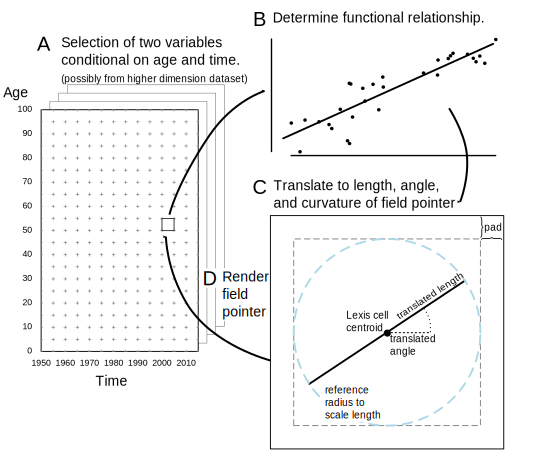
\includegraphics[scale=.8]{Figures/ExplainerDiagram.pdf}
  \caption{A diagram depicting the translation of functional relationships in data conditioned on age and time to visual encoding on a Lexis field. \textbf{A}: Condition data selection on age and time. \textbf{B}: model the functional relationship in data subset. \textbf{C}: Translate the model to field elements, `pointers', using angle, and possibly also length, curvature, thickness, etc to encode model qualities. \textbf{D}: Populate the Lexis plane with field pointers to create a Lexis field.}
  \label{fig:explain}
\end{figure}

\section{Application}
We offer a selection of variants of Lexis field design for our example of the relationship between the mean and standard deviation of remaining lifespan. The first of these, Figure~\ref{fig:sfig1}, is a bare-bones Lexis field that serves to illustrate the underlying concept. This display differs from a standard vector field in two notable ways. 1) Segments are drawn rather than arrows, because each slope can be
interpreted as a subplot, where the convention is to always read a
relationship from left to right. 2) The left and right extremes are fixed for
each segment according to the year-width rendered, in this case 5-year
groupings. This means that relationships farther from zero also result in longer
line segments, but the length of the line segment is not strictly proportional
to the magnitude of the slope coefficient or any other quantity. For each
subplot, the x range represents the same hypothetical range of
variation in remaining life expectancy or 2 years. The y-axis is arbitrarily,
but identically scaled for each subplot. Other criteria for slope length would
also be possible and will be considered.

Figure~\ref{fig:sfig2} is identical to the previous, but adds a red contour line
at the turning point in slopes. In this case there is only one sign change is slope
coefficients over the age pattern. It is easier to locate and detect change in
this (novel) threshold with the line markup than from the bare Lexis field.
Indeed one could add further isoclines at slope break points, as in
Figure~\ref{fig:sfig3} or \ref{fig:sfig4}, and insodoing we begin a transition
into the more standard graphical form of contour maps. Figure~\ref{fig:sfig3}
blends the Lexis field with a heatmap, where hue indicates both direction and
magnitude of slope coefficients. In this case, slope coefficients are
double-coded, and this display is likely the most legible, but it comes at a
cost of clutter. Figure~\ref{fig:sfig4} removes the slope segments, but is
otherwise identical. We wish to explore variants of the first three of these
Lexis field proposals, and may possibly display more example relationships
between other variables in a full manuscript, data permitting.

\begin{figure}
\begin{subfigure}{.5\textwidth}
  \centering
  \includegraphics[scale=.4]{Figures/FigApp1.pdf}
  \caption{A simple field.}
  \label{fig:sfig1}
\end{subfigure}%
\begin{subfigure}{.5\textwidth}
  \centering
  \includegraphics[scale=.4]{Figures/FigApp2.pdf}
  \caption{A simple field, with the zero-slope isocline drawn (red).}
  \label{fig:sfig2}
\end{subfigure}
\begin{subfigure}{.5\textwidth}
  \centering
  \includegraphics[scale=.4]{Figures/FigApp3.pdf}
  \caption{Slopes doubly coded with field segments and discrete color, further
  slope isoclines drawn.}
  \label{fig:sfig3}
\end{subfigure}%
%\begin{subfigure}{.5\textwidth}
%  \centering
%  \includegraphics[scale=.6]{Figures/Fig12-crop.pdf}
%  \caption{Discrete color heatmap with selected isoclines drawn.}
%  \label{fig:sfig4}
%\end{subfigure}
\caption{Four versions of Lexis fields displaying the linear
relationship between the standard deviation and mean of remaining
lifespan, males (HMD)}
\label{fig:fig}
\end{figure}

\section{Discussion}
Although patterns in data may be much more complex than can be expressed with linear models, these simple model fits can be thought of as regular samples from the complex space implied by data, such that the pattern revealed on the Lexis field is still inteligible. 


\nocite{vaupel1987thousands}

\FloatBarrier
\singlespacing
\bibliographystyle{plainnat}
  \bibliography{references} 

\end{document}
